\documentclass[twocolumn,10pt]{article}
\usepackage[greek,francais,english]{babel}
\usepackage[T1]{fontenc}
\usepackage[utf8]{inputenc}
\usepackage[top=2cm, bottom=2cm, left=1cm, right=1cm]{geometry}
\setlength{\columnsep}{1cm}
\usepackage[usenames,dvipsnames]{color}
\usepackage{graphicx}
%\usepackage{multicol}
\renewcommand{\rmdefault}{ptm}
\newcommand\tet{\textgreek{tetraf'armakos} }
\makeatletter
\newenvironment{tablehere}
  {\def\@captype{table}}
  {}
\newenvironment{figurehere}
  {\def\@captype{figure}}
  {}
\makeatother
%================
\begin{document}
\title{\tet %en cas de problème avec cette fonte, ne pas hesiter à enlever le \tet en le commentant avec un % suivit d'un passage à la ligne
: Vegetation, atmosphere\\ and flight parameters monitoring} 
\author{Clément Javerzac-Galy \and{Denis Savoie}\\
\texttt{cansat2012@supop.fr}
\and{Zubair Iftikhar}
}
\date{\today}
\maketitle
 
\begin{abstract}
    \begin{bfseries}
    \par The \tet \footnote{prononcez tetrapharmakos} is a Cansat project of the \textit{Proton-thérapeutes} team for the second participation of the Institut d'Optique \textit{Graduate School} to the \textit{C'Space} competition co-organised by Planète-Sciences and the CNES. 
    \par This space probe with bring a homemade module to detect chlorophile. It will also make an atmospheric sounding and position tracking during its fall.
    \par We hope these complementary studies could help to determine the chance of life on an Earth-like exoplanet.
     \end{bfseries}
\end{abstract}
\section{Introduction}%=========================================
    \par First of all, we need to precise that a Cansat is not really a satellite contained in a can. Indeed it will only fall instead of enter in any orbit. Then it is actually a space probe.
    \par We are making the \tet in order to participate to the competition a Cansat competition co-organised by \textit{Planète-Sciences} and the \textit{CNES} : the C'Space 2012. It have to fulfill 2 missions, one of which is free. For the imposed mission, we decided to do an atmospheric soudering. And our Fourier Optics professor Jean Taboury suggested us to make an NDVI measurment for the free mission.
    \par In addition to these 2 missions, an other aspect of our work is to build something consistent. That means a probe that can be contained in 33 cL, enough fast acquire a lot of informations, electically autonomous, entirely automatic during the flight and finally resistant to a 200m height fall --- using a parachute, of course.
\section{Context of developpement}%================================
    \subsection{Club}%&&&
    \par The \textit{Proton-thérapeutes} team is composed of 3 first-year MSc studuents at the Institut d'Optique \textit{Graduate School}. The first time our school participate to the Cansat competition was in 2011. This project has been initiated by Jean-Marie Feybesse, IT professor at Paris XI. But unfortunatly, this team\footnote{Archimede, leaded by Sébastien Guidicelli} didn't reached the last step of competition beacause of logistic issues.
    \par As the previous team, we are 3. This number is too little not to be aware of the work of the whole team. Each member has not a specific work. Nevertheless some leadings have emerged, then we can describe the team as the following list:
    \begin{itemize}
        \item Clément: mecanic and electronic chips designer
        \item Denis: electonics and cameras implementation
        \item Zubair: sensors implementation and parachute design
    \end{itemize}
    \subsection{Work plan}%&&&
\section{Definition of the missions}%================================
    \subsection{Proposed mission : Atmospheric sounding}%&&&
        \par We chose to measure the temperature, the humidity and the pressure during the fall of our cansat thanks to two electronic captors : the BMP085 that measures the temperature and the pressure, and the DHT22 that measures the temperature and the humidity. Measurements are made every two seconds, which is the refreshment rate of the used captors, and the requirement of the mission.
    \subsection{Free mission : chlorophyle detection}%&&&
        \par In this mission, we detect active chlorophyle by multispectral imagery.
        \paragraph*{Chlorophyll spectrum} Chlorophyll absorbs much red, and emits in near infrared.
        \begin{figure}[!h]
        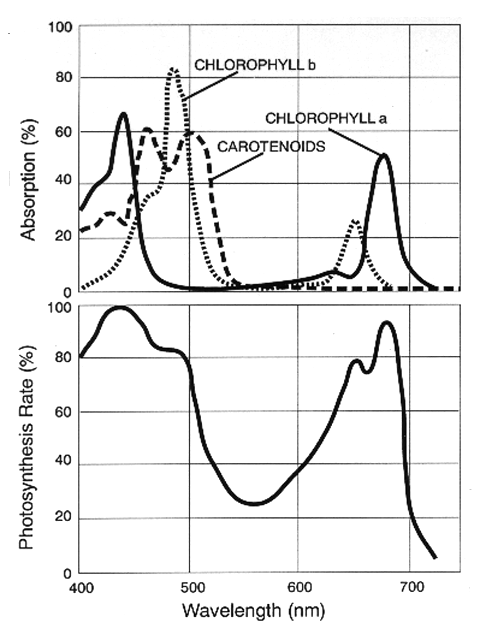
\includegraphics[scale=.4]{Par_action_spectrum.png}
        \caption{Absorption and fluorescence specrums of chlorophyll}
        \end{figure}
        \par So we use this by taking two pictures of the same scene, one in a red spectral band, the other in a near infrared spectral band. We then calculate the Normalized Difference Vegetation Index(NDVI) with this formula :
         \[ \textrm{NDVI} = \frac{\textrm{RED}-\textrm{NIR}}{\textrm{RED}+\textrm{NIR}} \]
        \paragraph*{Detection system} The images in red and in NIR bands are taken by two CCD. In order to detect red on one CCD, and NIR on the other, we use a cold mirror and filters. The hot mirror transmits most of visible light, and reflects most of infrared. Just like the chlorophyle its reflection and transmission spectrum cuts arround $700nm$. Just before the CCD, we put filters more selective filters. The use of the hot mirror allows to keep a better part of the flux for both bands than a simple beam splitter, and allows to cut infrared for the red detector. Before the hot mirror, we use a camera lens to form the image on both CCD, for instance we used a simple lens.
        \begin{figure}[!h]
        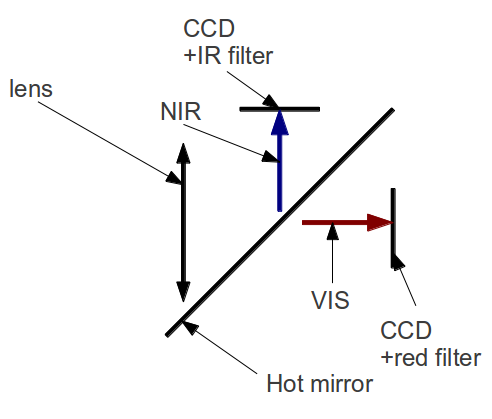
\includegraphics[scale=.5]{sch_opt.png}
        \caption{Schematic of the imagery system}
        \end{figure}
        \begin{figure}[!h]
        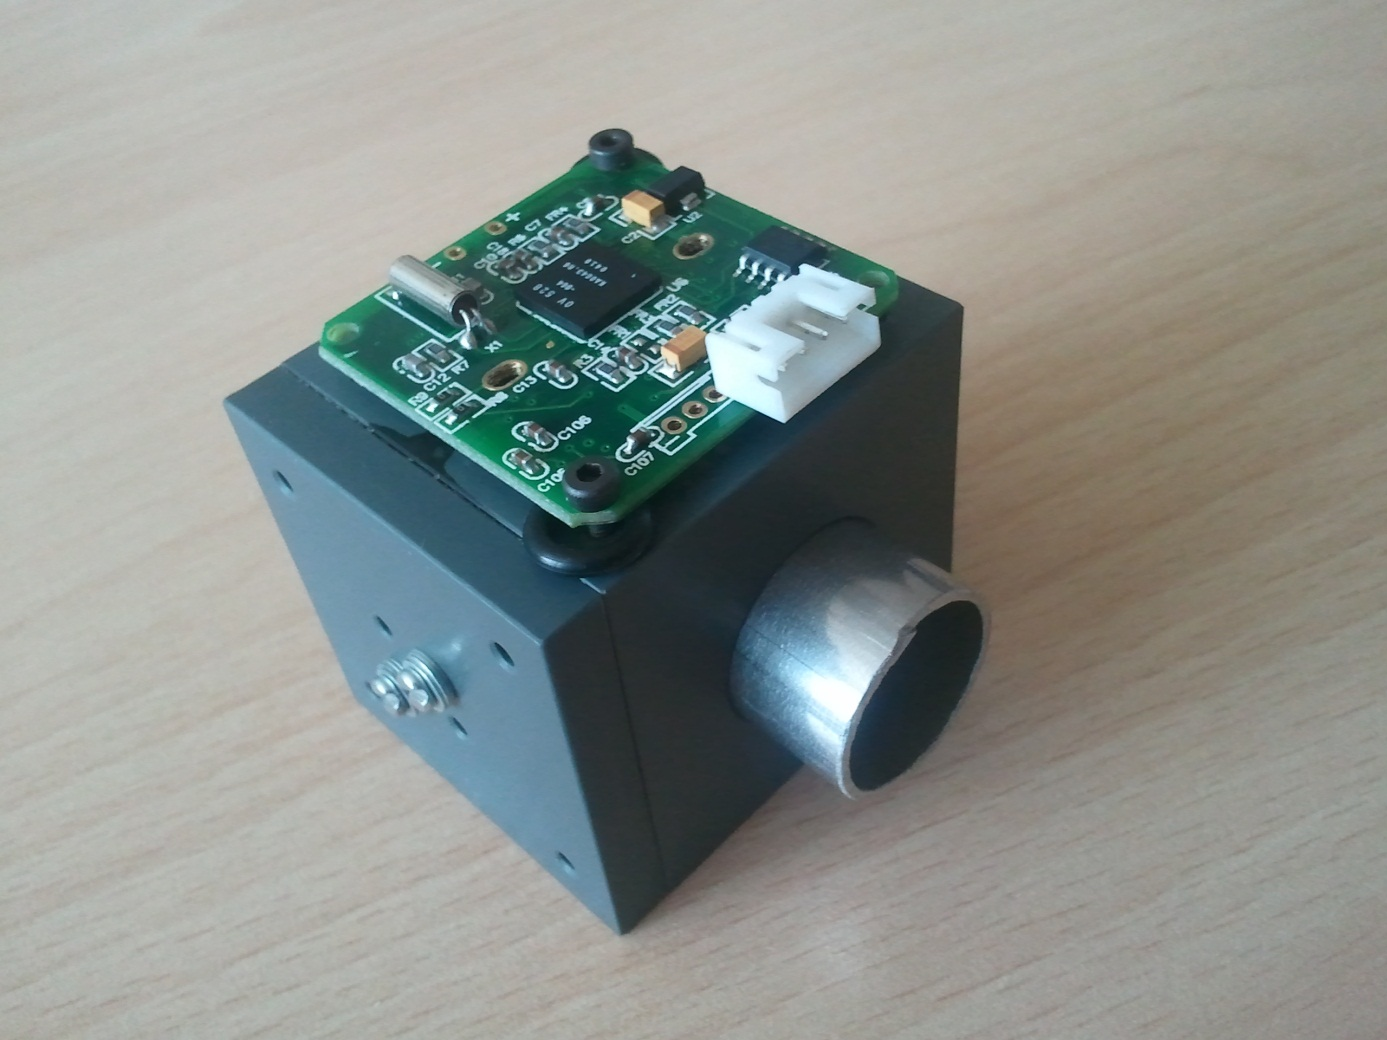
\includegraphics[scale=.5]{cube.png}
        \caption{Photograph of the assembled imagery system}
        \end{figure}
    \subsection{Additionnal measurements}%&&&
    \par We also track the position and the speed of the cansat thank to an accelerometer and a GPS. It will be useful to fit pressure measurments with a model. 
\section{Cansat architecture}%====================================
    \subsection{Electrical architecture}%&&&
    \subsection{Mecanical parts}%&&&
    \subsection{Telemetry}%&&&
    \subsection{Flight algorithm}%&&&
\section{Conclusion}%=========================================
\section*{Acknowledment}
\begin{thebibliography}{9}
  % la biblio
\end{thebibliography}
\end{document}

